\section{Software Structure}
\begin{figure}
\begin{center}
\begin{scriptsize}

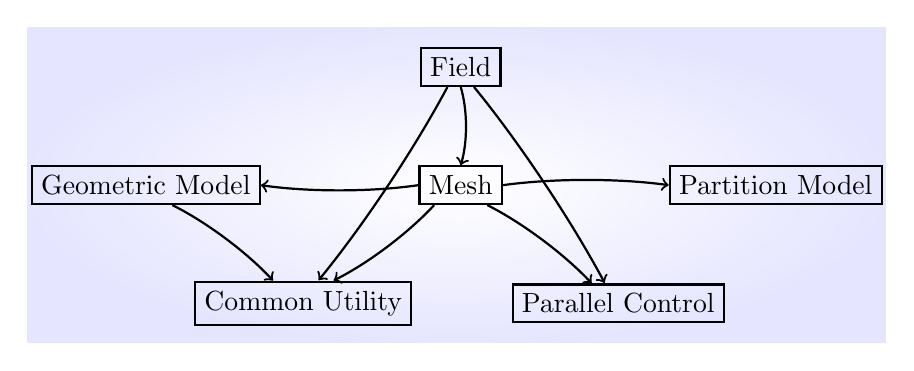
\begin{tikzpicture}[decoration={bent,aspect=.3}]
 \shade[outer color=blue!10!white, inner color=white] (-1.5,-0.5) rectangle 
(9.4,3.5);
 \node[rectangle,draw,thick] (F) at (4,3.0) {Field};
 \node[rectangle,draw,thick] (A) at (0,1.5) {Geometric Model};
 \node[rectangle,draw,thick] (B) at (4,1.5) {Mesh};
 \node[rectangle,draw,thick]  (C) at (8,1.5) {Partition Model};
 \node[rectangle,draw,thick]  (E) at (2,0) {Common Utility};
 \node[rectangle,draw,thick]  (D) at (6,0) {Parallel Control};
 \draw[->,decorate,thick] (A) -- (E);
 \draw[->,decorate,thick] (B) -- (A);
 \draw[->,decorate,thick] (B) -- (C);
 \draw[->,decorate,thick] (B) -- (D);
 \draw[->,decorate,thick] (B) -- (E);
 \draw[->,decorate,thick] (F) -- (B);
 \draw[->,decorate,thick] (F) -- (D);
 \draw[->,decorate,thick] (F) -- (E);
\end{tikzpicture}
\end{scriptsize}
\end{center}
\caption{PUMI components: an arrow from component $A$ to component $B$ indicates 
that the component $A$ is dependent on the component $B$}
\label{fig:pumi-comp}
\end{figure}

PUMI consists of six software components (Figure~\ref{fig:pumi-comp})~\cite{pumi12,pumiweb}: 
\emph{(i)} the Common Utility for common tools and services used in multiple other 
components, \emph{(ii)} the Parallel Control component for parallel-specific tools 
and services, \emph{(iii)} the Geometric Model component for interfacing with geometric
 model kernels, \emph{(iv)} the Mesh component to provide the distributed mesh 
representation and manipulations, \emph{(v)} the Partition Model component for 
partition model representation and manipulations, and 
\emph{(vi)} the Field component for field storage and manipulations.

As a partition model is constructed based on the mesh distribution, it is
 automatically updated when mesh partitioning is changed. Therefore its functionality is 
embedded in mesh implementation and furthermore, access/modification 
by the users is not needed. 
Except for the Partition Model component, each component is a self-contained, 
independently usable library with its own set of requirements and 
well-defined API. 

\subsection{pcu - Parallel Control Utility Library}
\emph{pcu} is a library that provides a parallel programming model including 
parallel control functions.
Its two major functionalities are \emph{message passing} that allows parallel tasks to 
coordinate and \emph{thread management} that extends the MPI programming model 
into a hybrid MPI/thread system.

The foundation of \emph{pcu} is its point-to-point message passing routines where 
non-blocking synchronous message passing primitives are defined. There are 
two versions, one of which is a direct interface to MPI, and the second supports 
message passing between threads~\cite{dan-supcomp14}. The two versions 
are interchangeable, and \emph{pcu} can change which set of them is being used at 
run-time without affecting the rest of software components.

Building on the point-to-point primitives, \emph{pcu} has an extensible framework for
collective operations such as reduction, broadcast, scan, and barrier.
Any collective whose communication pattern can be encoded as some kind of tree
is supported, and the most common ones come built-in to \emph{pcu}.
These collectives are directly available to users.

Using both collectives and point-to-point communication, \emph{pcu} provides a message 
passing algorithm for general unstructured communication. The \emph{send} phase 
allows tasks to send any messages out to neighbors and 
the \emph{receive} phase ensures that neighbors 
receive all the messages they have been sent. This \emph{phased} communication algorithm is 
equivalent to the non-blocking consensus algorithm
for sparse data exchange~\cite{hoefler2010scalable}.
%This \emph{phased communication} API is the part of \emph{pcu} used most heavily by the 
%mesh database and other users.

Finally, \emph{pcu} has a system for creating a pool of threads within each process and 
assigning them ranks the way MPI does to processes.
Users can call this API to enter a hybrid MPI/thread mode in which all the 
communication APIs (point-to-point, collective, and phased) work between 
threads. These capabilities support a hybrid MPI/thread operation.

\subsection{gmi - Geometric Model Interface Library}

The problem domain is the basis for generating meshes on 
which the analysis is performed. 
Commercial geometric modeling kernels such as Acis~\cite{acisweb}, 
Parasolid~\cite{parasolidweb} and GeomSim~\cite{geomsimweb}, provides the
description of the problem domain.

The geometric model library provides modeling 
kernel-independent geometry access by polymorphism and 
replicating the topological information 
 in modeling kernels. Therefore geometry-based applications 
(including mesh) can interface with various modeling 
kernels through geometric model library~\cite{vgi97,cgm01,beall-geom04}. 
In \emph{gmi}, the geometric 
model class hierarchy is derived for implementation with specific commercial 
geometric modeling kernels such as Acis~\cite{acisweb}, GeomSim~\cite{geomsimweb}, and 
Parasolid~\cite{parasolidweb}. In case of no 
commercial modeling kernel available, \emph{gmi} supports a geometric model 
constructed from mesh, called \emph{mesh model}~\cite{beall-geom04}.
The following core functionalities are provided at the high-level API 
regardless of underlying modeling kernel.


\begin{enumerate}
\item[-] \emph{modeling kernel registration and importing} - 
establishing the relationship between the high-level API 
and the modeling kernel specific API and importing 
the geometric model information into topological representation.
\item[-] \emph{geometric model representation} - maintaining pointers to 
topological model entities. In boundary representation, they are regions, 
shells, faces, loops, edges, vertices and \emph{use} entities for vertices, 
edges, loops, and faces with a non-manifold model~\cite{weiler88}. The 
information stored in these data structures provide topological definition of 
the geometric model, so the mesh structure can always be correctly classified 
and the topological similarity between the mesh and the model can be maintained 
during modifications.
%\item[-] \emph{tagging} - attaching user data of various types (single or array 
%of integer, pointer, floating point, binary, set, entity) to model entity
%\item[-] \emph{traversal} - model entity traversal by dimension
%\item[-] \emph{entity set} - grouping arbitrary set of model entities
\item[-] \emph{interrogations} - adjacency, tolerance, and shape information, 
etc. Model entity objects themselves contain boundary-representation adjacency 
structures to other model entities as well as declaring virtual methods for 
modeler queries such as evaluating a point of a parametric
surface~\cite{beall-geom04}.
\end{enumerate}

Recently, models with thousands to millions of model entities are being 
constructed in \emph{gmi}, which prompted the addition of fast lookup 
structure to the model object since retrieval of a model entity from its integer 
identifier is a common operation during message passing and file reading. 

\subsection{mds - Mesh Data Structure Library}\label{sec:pumi_mesh}

An efficient 
and scalable distributed mesh data structure is  mandatory to achieve 
performance since it strongly influences the overall performance of adaptive 
mesh-based simulations. In addition to the general mesh-based operations, the 
distributed mesh data structure must support \emph{(i)} efficient communication 
between entities duplicated over multiple processes, \emph{(ii)} migration of 
entities or group of entities between parts, \emph{(iii)} dynamic load 
balancing. \emph{mds} provides the storage and management of distributed 
unstructured meshes and partition model. It supports all the mesh-level services to interrogate/modify 
the mesh data needed by parallel adaptive analysis. 
Core \emph{mds} functionalities include:

\begin{figure}
\begin{center}
\begin{scriptsize}
\begin{tikzpicture}
%distributed mesh
%\node[circle,fill] (0) at (0,0) {};
%\node[circle,fill] (1) at (1.1,0){};
%\node[circle,fill] (2) at (2,0) {};
%\node[circle,fill] (3) at (3,0) {};
%\node[circle,fill](4) at (0,0.8) {};
%\node[circle,fill](5) at (0.9,0.9) {};
%\node[circle,fill](6) at (1.9,0.85) {};
%\node[circle,fill](7) at (3,0.8) {};
%\node[circle,fill](8) at (0,1.7) {};
%\node[circle,fill](9) at (0.8,2.1) {};
%\node[circle,fill](10) at (1.7,1.6) {};
%\node[circle,fill](11) at (3,1.7) {};
%\node[circle,fill](12) at (2,2.4) {};
%\node[circle,fill](13) at (0,3) {};
%\node[circle,fill](14) at (1.6,3) {};
%\node[circle,fill](15) at (3,3) {};

%p_0

%\node[circle,fill](4) at (-.1,0.7) {};
%\node[circle,fill](5) at (0.8,0.8) {};
%\node[circle,fill](8) at (-.1,1.6) {};
%\node[circle,fill](9) at (0.7,2) {};
%\node[circle,fill](10) at (1.6,1.5) {};
%\node[circle,fill](13) at (-.1,2.9) {};
\draw[-,decorate] (-.2,0.7)--(0.7,0.8);%(4)-(5)
\draw[-,blue!80!green,line width=2pt,decorate] (-.2,0.7)--(-.2,1.6);%(4)-(8)
\draw[-,decorate] (0.7,0.8)--(-.2,1.6);%(5)-(8)
\draw[-,decorate] (0.7,0.8)-- (0.6,2);%(5)-(9)
\draw[-,decorate] (0.7,0.8)--(1.5,1.5);%(5)-(10)
\draw[-,decorate] (-.2,1.6)-- (0.6,2);%(8)-(9)
\draw[-,blue!80!green,line width=2pt,decorate] (-.2,1.6)--(-.2,2.9);%(8)-(13)
\draw[-,decorate] (0.6,2)--(1.5,1.5);%(9)-(10)
\draw[-,decorate] (0.6,2)--(-.2,2.9);%(9)-(13)
\node[blue!80!green] at(-1.4,1.7){$P_0$};
\node at (-.6,2.9){$M^0_1$};
\draw[inner color=white, thick] (-.2,2.9) circle (3pt);
\node at (-.6,1.6){$M^0_2$};
\draw[fill, inner color=gray, thick] (-.2,1.7)--(-.33,1.5)--(-.097,1.5)--cycle;
\node at (-.6,.7){$M^0_3$};
\draw[inner color=white, thick] (-.3,.6) rectangle (-.1,.8);

%p_1
\node[blue!80!green] at(.7,-.9){$P_1$};
%\node[circle,fill] (0) at (-.1,-.4) {};
%\node[circle,fill] (1) at (1,-.4){};
%\node[circle,fill] (2) at (1.9,-.4) {};
%\node[circle,fill](4) at (-.1,0.4) {};
%\node[circle,fill](5) at (0.8,0.5) {};
%\node[circle,fill](6) at (1.8,0.45) {};
%\node[circle,fill](10) at (1.6,1.2) {};
\draw[-,decorate] (-.1,-.4)--(1,-.4);%(0)-(1)
\draw[-,blue!80!green,line width=2pt,decorate] (-.1,-.4)--(-.1,0.4);%(0)-(4)
\draw[-,decorate] (1,-.4)--(1.9,-.4);%(1)-(2)
\draw[-,decorate] (1,-.4)--(-.1,0.4);%(1)-(4)
\draw[-,decorate] (1,-.4)--(0.8,0.5);%(1)-(5)
\draw[-,decorate] (1,-.4)--(1.8,0.45);%(1)-(6)
\draw[-,decorate] (1.9,-.4)--(1.8,0.45);%(2)-(6)
\draw[-,decorate] (-.1,0.4)--(0.8,0.5);%(4)-(5)
\draw[-,decorate] (0.8,0.5)--(1.8,0.45);%(5)-(6)
\draw[-,decorate] (0.8,0.5)--(1.6,1.2);%(5)-(10)
\draw[-,decorate] (1.8,0.45)--(1.6,1.2);%(6)-(10)
\node at (-.5,.3){$M^0_3$};
\draw[inner color=white, thick] (-.2,.3) rectangle (0,.5);
\node at (-.5,-.4){$M^0_4$};
\draw[fill, inner color=gray, thick](-.1,-.4) circle (3pt);

%line between processes
\draw[-,red!75!black, dotted, line width=1pt, decorate] 
(0.8,2.1)--(1.7,1.55);%(9)-(10)
\draw[-,red!75!black,dotted, line width=1pt, decorate] 
(0.8,2.1)--(0,3);%(9)-(13)
\draw[-,red!75!black, dotted,line width=1pt, decorate] 
(0,3)--(-0.7,3.5);%(13)-()
\draw[-,red!75!black, dotted,line width=1pt, decorate] 
(1.7,1.55)--(1.95,0.55);%(10)-(6)
\draw[-,red!75!black, dotted,line width=1pt, decorate] 
(1.95,0.55)--(2.05,-.4);%(6)-(2)
\draw[-,red!75!black, dotted,line width=1pt, decorate] 
(2.05,-.4)--(2,-0.9);%(2)-()

%p_2
%\node[circle,fill] (2) at (2.2,-.2) {};
%\node[circle,fill] (3) at (3.2,-.2) {};
%\node[circle,fill](6) at (2.1,0.65) {};
%\node[circle,fill](7) at (3.2,0.6) {};
%\node[circle,fill](10) at (1.9,1.4) {};
%\node[circle,fill](11) at (3.2,1.5) {};
%\node[circle,fill](12) at (2.2,2.2) {};
%\node[circle,fill](14) at (1.8,2.8) {};
%\node[circle,fill](15) at (3.2,2.8) {};
\draw[-,decorate] (2.2,-.2)--(3.2,-.2);%(2)-(3)
\draw[-,decorate] (2.2,-.2)--(2.1,0.65);%(2)-(6)
\draw[-,decorate] (2.2,-.2)--(3.2,0.6);%(2)-(7)
\draw[-,blue!80!green,line width=2pt,decorate] (3.2,-.2)--(3.2,0.6);%(3)-(7)
\draw[-,decorate] (2.1,0.65)--(3.2,0.6);%(6)-(7)
\draw[-,decorate] (2.1,0.65)--(1.9,1.4);%(6)-(10)
\draw[-,decorate] (3.2,0.6)-- (1.9,1.4);%(7)-(10)
\draw[-,blue!80!green,line width=2pt,decorate] (3.2,0.6)--(3.2,1.5);%(7)-(11)
\draw[-,decorate] (1.9,1.4)--(3.2,1.5);%(10)-(11)
\draw[-,decorate] (1.9,1.4)--(2.2,2.2);%(10)-(12)
\draw[-,decorate] (3.2,1.5)--(2.2,2.2);%(11)-(12)
\draw[-,blue!80!green,line width=2pt,decorate] (3.2,1.5)--(3.2,2.8);%(11)-(15)
\draw[-,decorate] (2.2,2.2)--(3.2,2.8);%(12)-(15)
\node at(5.1,1.3){$M^1_j$ $\sqsubset$ $G^1_j$};
\draw[->,thick,decorate] (4.5,1.3)--(3.2,2.2);%(G)-(11)
\draw[->,thick,decorate] (4.5,1.3)--(3.2,.95);%(G)-(11)
\draw[->,thick,decorate] (4.5,1.3)--(3.2,.1);%(G)-(11)

\node[blue!80!green] at (4.5,.7){$P_2$};
\node at (3.6,2.7){$M^0_5$};
\draw[inner color=white, thick] (3.2,2.7) circle (3pt);
\node at (3.6,1.5){$M^0_6$};
\draw[inner color=gray, thick] (3.2,1.6)--(3.08,1.4)--(3.32,1.4)--cycle;
\node at (3.6,.75){$M^0_7$};
\draw[inner color=white, thick] (3.1,.5) rectangle (3.3,.7);
\node at (3.6,-.3){$M^0_8$};
\draw[fill, inner color=gray,thick] (3.2,-.2) circle (3pt);

%p_3
%\node[circle,fill](9) at (0.9,2.2) {};
%\node[circle,fill](10) at (1.8,1.7) {};
%\node[circle,fill](12) at (2.1,2.5) {};
%\node[circle,fill](13) at (0.1,3.1) {};
%\node[circle,fill](14) at (1.7,3.1) {};
%\node[circle,fill](15) at (3.1,3.1) {};

\draw[-,decorate] (0.9,2.2)--(1.8,1.7);%(9)-(10)
\draw[-,decorate] (0.9,2.2)--(2.1,2.5);%(9)-(12)
\draw[-,decorate] (0.9,2.2)--(0.1,3.1);%(9)-(13)
\draw[-,decorate] (0.9,2.2)--(1.7,3.1);%(9)-(14)
\draw[-,decorate] (1.8,1.7)--(2.1,2.5);%(10)-(12)
\draw[-,decorate] (2.1,2.5)--(1.7,3.1);%(12)-(14)
\draw[-,decorate] (2.1,2.5)--(3.1,3.1);%(12)-(15)
\draw[-,decorate] (0.1,3.1)--(1.7,3.1);%(13)-(14)
\draw[-,decorate] (1.7,3.1)--(3.1,3.1);%(14)-(15)
\node[blue!80!green] at(1.5,3.5){$P_3$};
\node at(.1,3.4){$M^0_1$};
\draw[inner color=white, thick] (.2,3.1) circle (3pt);
\node at(3.1,3.4){$M^0_5$};
\draw[inner color=white, thick] (3.1,3.1) circle (3pt);

\node[red!75!black] at (-1.9,2.4){{$PROCESS$ $i$}};
\node at (-2.2,.8){$M^1_i$ $\sqsubset$ $G^1_i$};
\draw[->,thick,decorate] (-1.6,.8)--(-.2,2.4);%(G)-(14)
\draw[->,thick,decorate] (-1.6,.8)--(-.2,1.2);%(G)-(14)
\draw[->,thick,decorate] (-1.6,.8)--(-.1,-.15);%(G)-(14)

\node[red!75!black] at(5,2){{$PROCESS$ $j$}};

\end{tikzpicture}
\end{scriptsize}
\end{center}
\caption[Distributed mesh on two processes with matching]{2D distributed mesh 
with periodic model edges $G^1_i$ and $G^1_j$}
\label{fig:matching}  % the \label command comes AFTER the caption
\end{figure}

\begin{enumerate}
%1
\item[-] \emph{interrogations} - $1^{st}$ and $2^{nd}$-order adjacency,
 owning part, status (internal, part boundary, matched, 
ghost or ghosted), classification (geometric and partition model), etc.
%2
\item[-] \emph{modification} - entity and set creation/deletion, migrating 
entity and p-set from part to part including tagged data, 
and a capability to dynamically change the number of parts per process.
%\item[-] migration: it is performed frequently to support
% \emph{(i)} distribute the mesh to parts, 
%(ii) keep the mesh load balancing, and
%\emph{(iii)} obtain needed mesh entities for local mesh modification.
%~\cite{fmdb06,adapt06}.
%3
\item[-] \emph{load-balancing} -  a capability 
to balance the mesh load on each part predictively~\cite{predictive97,zhou12} or 
as post-processing with the help of mesh migration and partitioning libraries 
such as Zoltan, ParMETIS, and ParMA. Zoltan is a toolkit for scientific 
applications and it provides
graph-based load balancing and partitioning algorithms~\cite{zoltanweb}.
ParMETIS provides algorithms for partitioning unstructured graphs, meshes, and 
for computing fill-reducing orderings of sparse matrices~\cite{parmetisweb}.
ParMA is a partitioning library developed at SCOREC without using
 the classical graph data structure. Three ParMA procedures are \emph{(i)} multi-criteria 
diffusive partition improvement~\cite{zhou-contr,zhou-extr}, 
\emph{(ii)} predicted load balancing~\cite{predictive97,zhou12}, 
and \emph{(iii)} heavy part splitting~\cite{zhou12,pumi12}. 

%4
\item[-] \emph{matching} - a capability to maintain mesh entities on matched, 
periodic model boundaries~\cite{matching07,meshsimmatchingweb}. 
Figure~\ref{fig:matching} illustrates four-part distributed mesh with periodic 
model edges $G^1_i$ and $G^1_j$ (thick solid lines). The mesh entities 
classified on $G^1_i$ are matched to mesh entities classified on $G^1_i$, vice 
versa. For instance, $M^0_1@P_0$ is matched to three mesh vertices, $M^0_1@P_3$, 
$M^0_5@P_3$, and $M^0_5@P_2$. $M^0_3@P_0$ is matched to two mesh vertices, 
$M^0_3@P_1$, and $M^0_7@P_2$. When a mesh entity is modified or migrated, all 
the matched copies should be updated as well to keep the identity.
%5
\item[-] \emph{file I/O} - ascii or binary file I/O in various mesh formats 
(NetCDF~\cite{netcdfweb}, Exodus~\cite{exodusreport94}, VTK~\cite{vtkweb}, 
Simmetrix~\cite{simmetrixweb}, etc.) for partition model and mesh entities with 
auxiliary data including geometric classification, partition classification, 
tagged data, entity sets~\footnote{grouping of arbitrary entities from multiple 
parts or a single part~\cite{moabreport04,imesh10,itapsweb}.}, matched copies, etc.
\end{enumerate}

\begin{figure}
\begin{center}
\begin{scriptsize}
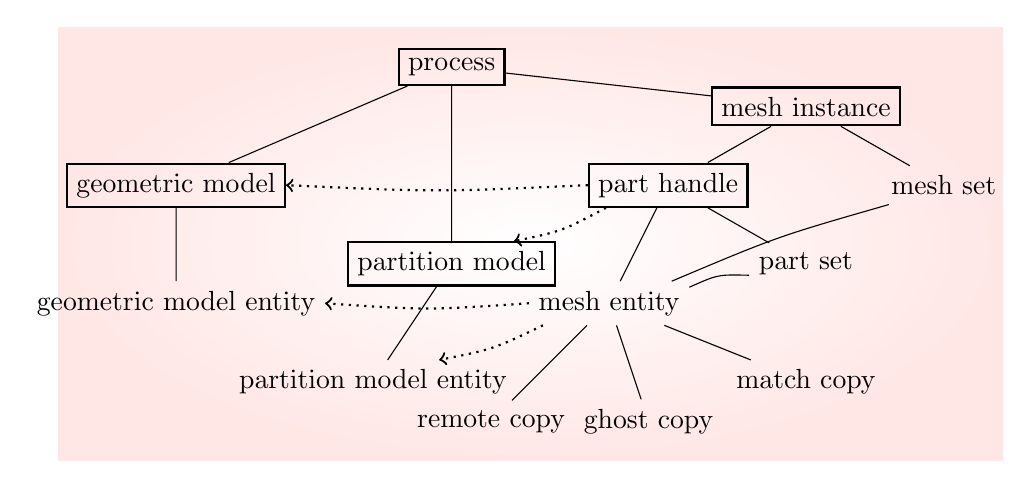
\begin{tikzpicture}[decoration={bent,aspect=.5}]
\shade[outer color=orange!10!red!10!white, inner color=white] (-5,.5) rectangle 
(7,-5);
 \node[rectangle,draw,thick]{process}
  child {node[rectangle,draw,thick] at (-2,0) (a) {geometric model}    child 
{node at (0,0) (b) {geometric model entity}}}
  child {node[rectangle,draw,thick] at (0,-1) (c) {partition model}    child 
{node at (-1,0) (d) {partition model entity}}}
  child {node[rectangle,draw,thick] at (3,1) (e) {mesh instance}    child 
{node[rectangle,draw,thick] (f) at (-1,0.5) {part handle}
                child {node (g) at (0,0){mesh entity}
                        child {node at (0,0){remote copy}}
                        child {node at (.5,0){ghost copy}}
                        child {node at (1,.5){match copy}}
                }
                child {node  (h) at (1,.5) {part set}}
        }
        child {node at (1,.5) (i) {mesh set}}}
  ;
 \draw[-,decorate] (g) -- (h);
 \draw[-,decorate] (g) -- (i);
 \draw[->,decorate,thick,dotted] (f) -- (a);
 \draw[->,decorate,thick,dotted] (f) -- (c);
 \draw[->,decorate,thick,dotted] (g) -- (d);
 \draw[->,decorate,thick,dotted] (g) -- (b);
% \draw[->,decorate,thick,dotted] (D) -- (B);
\end{tikzpicture}
\end{scriptsize}
\end{center}
\caption{Mesh data in process: A solid line from upper positioned component $U$ 
to lower positioned component $L$ indicates that the component $U$ contains 0 or 
more component $L$. A dotted arrow from component $A$ to component $B$ indicates 
that the component $A$ maintains a link to component $B$. A data drawn with 
rectangle indicates that at least one copy of the data should exist on each 
process.}
\label{fig:pumi-datamodel}
\end{figure}

The term 
\emph{instance} is used to indicate the model's data object existing on each process. For 
example, a mesh instance on a process means a pointer to a mesh data structure 
on the process and all parts on the process are maintained by, and accessible 
through, the mesh instance. The term \emph{handle} is used to indicate the 
pointer to the other types of data object such as part, entity and entity set. For example, a 
mesh entity handle means a pointer to the mesh entity data~\cite{fmdb06,imesh10,pumi12,itapsweb}. 
